\chapter{Method}
\label{ch:method}

\section{Architecture}

\begin{figure}[htp]
	\centering
	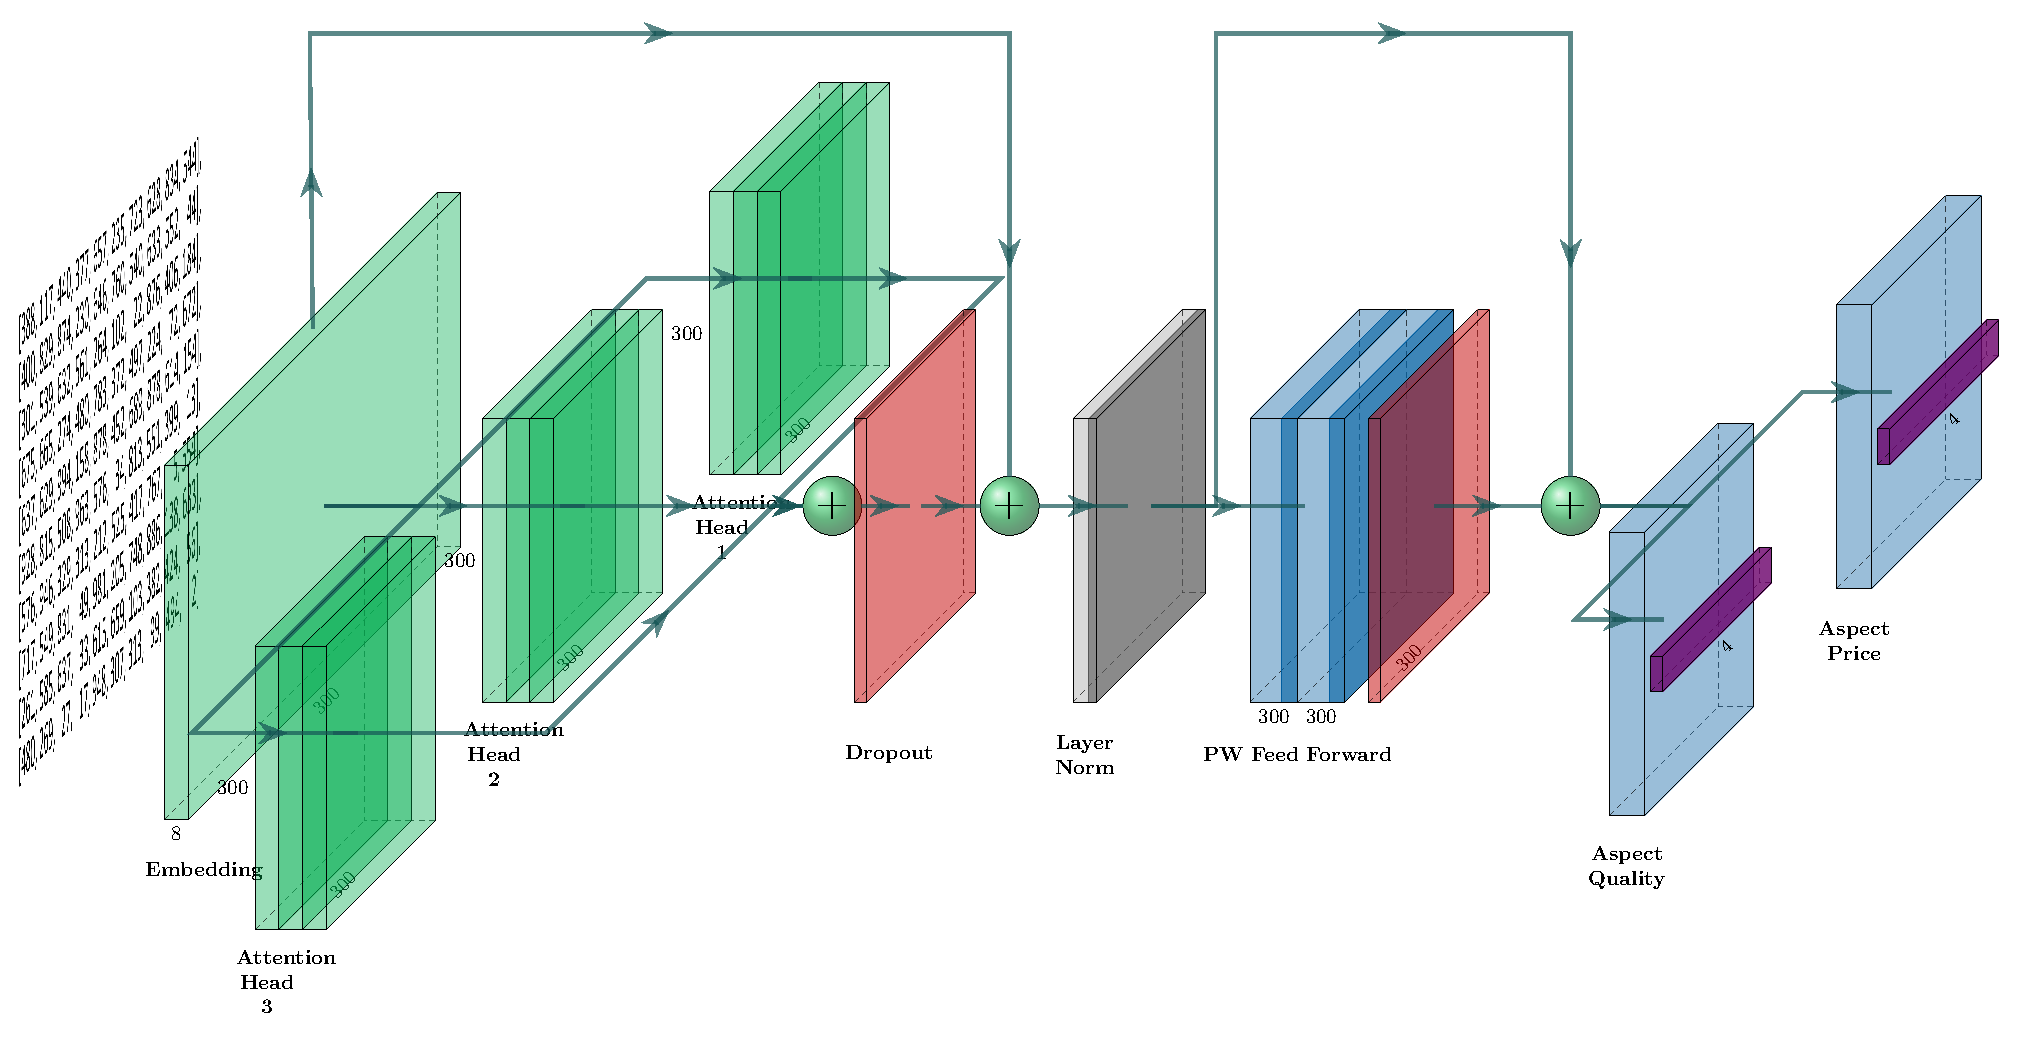
\includegraphics[width=\textwidth]{figures/04_method/04_t-absa}
	\caption{}
	\label{fig:04_t-absa}
\end{figure}

\subsection{Transformer}

\subsection{Aspect Heads}

\subsubsection{Linear Mean-Head}

why mean? -> bring loss to similar value regardless of a) word length and b) aspect head choice (linear vs cnn)

\subsubsection{Projection Mean-Head}

\subsubsection{CNN-Head}

\subsubsection*{Weighted Loss}

\begin{equation}
\mathcal{L}_\text{NLL}=-\frac{1}{n}\sum_{i=1}^{n} w_i * (y_i \cdot log(\hat{y}_i))
\label{eq:04_nll}
\end{equation}

where $n$ is the number of classes, $w_i$ is the class weight, $y_i$ is the ground truth and $\hat{y}_i$ is the prediction.

\section{Multi-Task Learning}

The way the \gls{absa}-Transformer is build, inevitably necessitates multi-task learning since for each aspect-head a separate \gls{nll}-loss is computed. For each of the $m$ classes a loss value is calculated. In the end the mean of all losses is taken as shown in equation \ref{eq:04_multiheadLoss}.

\begin{equation}
\mathcal{L}_\text{MultiTask} = \frac{1}{m}\sum_{j=1}^{m}\mathcal{L}(f(x), y_m)
\label{eq:04_multiheadLoss}
\end{equation}

where $\mathcal{L}(f(x), y_m)$ is the \gls{nll}-loss of the model $f$ with input the $x$.

\subsection*{Multitask Task Data Augmentation}

As described in section \ref{sec:03_mtlAdvantages} it is also possible to augment the data by using an auxiliary task in addition to the regular classification tasks.

There are three possible auxiliary tasks to consider:


\begin{enumerate}
	\item Predict additional label from the source data
	\item Use an additional dataset B in combination with the source dataset A and predict labels for the classes in A and the classes in B simulatanously. This approach is similar to transfer learning but instead of training the models sequentially, this approach would train them together.
	\item Predict additional aspects of the source data which can be trained unsupervised.
\end{enumerate}

This thesis will focus on the first type of auxiliary task where we will try predict an additional label for the source dataset. As the source dataset we choose the GermEval-2017 data since this dataset provides an additional document-wide sentiment label. This label was choosen since the other aspect heads already perform sentiment ananlisis so this task is very similar on the one hand but can provide additional datapoints for the training of the model. In addition the dataset provides a reasonable amnount of training data.

Training with the auxiliary sentiment label is performed by adding an additional sentiment head to the model.

%We also experiment with the weighting of the tasks in the loss


\section{Transfer Learning}

comparison to image first layer features which are very similar regardless of target domain. \cite{Yosinski2014} -> Embedding layer, Transformer

However, last layer usually very dependet on domain and dataset -> good for model because last layer -> heads only domain relevant. So keep Embedding and transformer and exchange heads.

